\documentclass{article}
\usepackage{amsmath}
\usepackage{amssymb}
\usepackage{tikz}
\usetikzlibrary{arrows.meta}

\begin{document}

\begin{figure}[h]
    \centering
    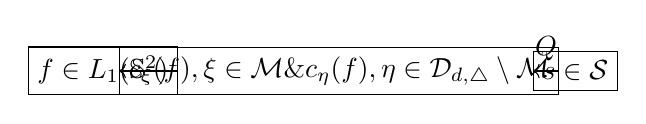
\begin{tikzpicture}[node distance=2cm, auto]
        % Define nodes
        \node[draw] (f) {$f \in L_1(\mathbb{S}^2)$};
        \node[draw, right of=f, node distance=3cm] (c) {$c_\xi(f), \xi \in \mathcal{M}$ \\ \& \\ $c_\eta(f), \eta \in \mathcal{D}_{d,\triangle} \setminus \mathcal{M}$};
        \node[draw, right of=c, node distance=3cm] (s) {$s \in \mathcal{S}$};
        
        % Draw edges
        \path[->] (f) edge node {} (c);
        \path[->] (c) edge node [above] {$Q$} (s);
    \end{tikzpicture}
    
    \caption{Illustration of quasi-interpolation operator $Q$. Here $c_\xi(f) = \gamma_\xi(F_{d,\tau_\xi} f)$ is the B-coefficients corresponding to $\xi$, $\tau_\xi$ is the triangle that contains $\xi$, $F_{d,\tau_\xi} f$ is the averaged Taylor polynomial of degree $d$ associated with $\tau_\xi$; $c_\eta(f)$ is a linear combination of $\{c_\xi(f)\}_{\xi\in\mathcal M_\eta}$, $\mathcal M_\eta \subseteq \text{star}^\curlywedge (\tau_\eta)$, $\tau_\eta$ is the triangle that contains $\eta$.}
    \label{fig:quasi_interpolation_operator}
\end{figure}

\end{document}